%     Compiler: pdflatex

\documentclass[12pt,a4paper]{article}
\usepackage{amsmath, amssymb}
\usepackage[utf8]{inputenc}
\usepackage[T1]{fontenc}
\usepackage[english]{babel}
\usepackage{graphicx}
\usepackage[margin=0.5in]{geometry}
\usepackage{float}

\graphicspath{{fig/}}

\title{MF2007 - Workshop A}

\author{
Adam Lang \\ 861110-3956
\and
Gabriel Andersson Santiago \\ 910706-4538
\and 
Andreas Fr\"oderberg \\ 880730-7577
}

\begin{document}
\maketitle

\section*{Parameter identification}

\subsection*{Level 1}
The parameters that was modeled originally was not very good and in
table \ref{tab:parameters} both the original and new parameters is
given.
\begin{center}
  \begin{table}[H]
    \caption{Parameters for the DC-motor}
    \begin{tabular}{|c|c|c|c|}
        \hline
        & Inertia & Coulomb Friction & Viscous Friction \\ 
        \hline
        Original & $2.18e^{-6}$ & $-$ & $3.8e{-6}$ \\
        \hline
        Adjusted & $2.5e^{-5}$ & $-$ & $2e^{-5}$ \\
        \hline
    \end{tabular}
   \label{tab:parameters}
  \end{table}
\end{center}
After adjusting the parameters, the result in figure
\ref{fig:par_level1} was obtained. We can
tune the model very good when modeling towards one velocity, but when
the velocity is changed, the model will differ from reality.
\begin{center}
    \begin{figure}[H]
    \centering
      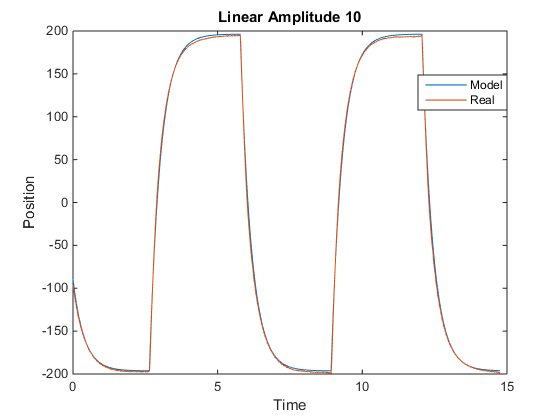
\includegraphics[scale = 0.6]{par_level1.png}
      \caption{The velocity output for the model and the real motor}
      \label{fig:par_level1}
    \end{figure}
\end{center}

\subsection*{Level 2}
The parameters from Level 1 and the coulomb friction can be seen in
table \ref{tab:parametersL2}.
\begin{center}
  \begin{table}[H]
    \centering
    \caption{Complete parameters for the DC-motor}
    \begin{tabular}{|c|c|c|c|}
        \hline
        & Inertia & Coulomb Friction & Viscous Friction \\ 
        \hline
        Original & $2.18e^{-6}$ & $1e^{-3}$ & $3.8e{-6}$ \\
        \hline
        Adjusted & $2.22e^{-5}$ & $8e^{-4}$ & $2e^{-5}$ \\
        \hline
    \end{tabular}
   \label{tab:parametersL2}
  \end{table}
\end{center}
When the model is changed to include coulomb friction it is still
equally easy to model for on single velocity, but it is easier to get
good results for different amplitudes. These results can be seen in
figure \ref{fig:par_level2}.
\begin{center}
  \begin{figure}[H]
    \centering
    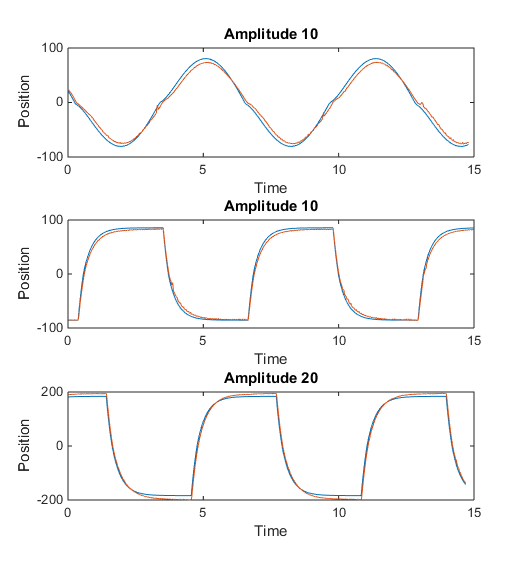
\includegraphics[scale=0.6]{par_level2.png}
    \caption{Velocity output for the model when including coulomb
    friction for sinus- and square wave input}
    \label{fig:par_level2}
    \end{figure}
\end{center}

\section*{Velocity Control}
  \subsection*{Level 1}
  The calculated control law is given by ...
  With the calculated control law we get the response seen in figure
  \ref. Here we can see that the requirements are met with no overshoot
  ant a maximum steady state error of $0.5$
  \begin{center}

      \begin{figure}[H]
        \centering
        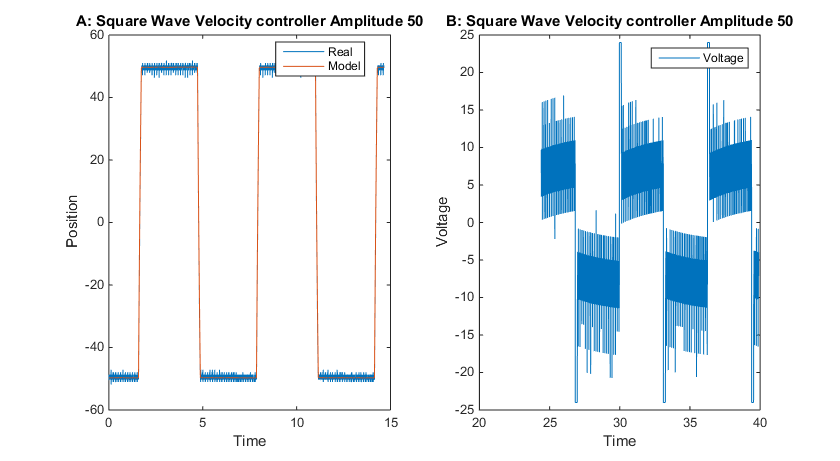
\includegraphics[scale=0.5]{41SqVo.png}
        \caption{A: Square wave response, B: Voltage }
        \label{fig:41SqVo}
      \end{figure}
      
      
      
      \begin{figure}[H]
        \centering
        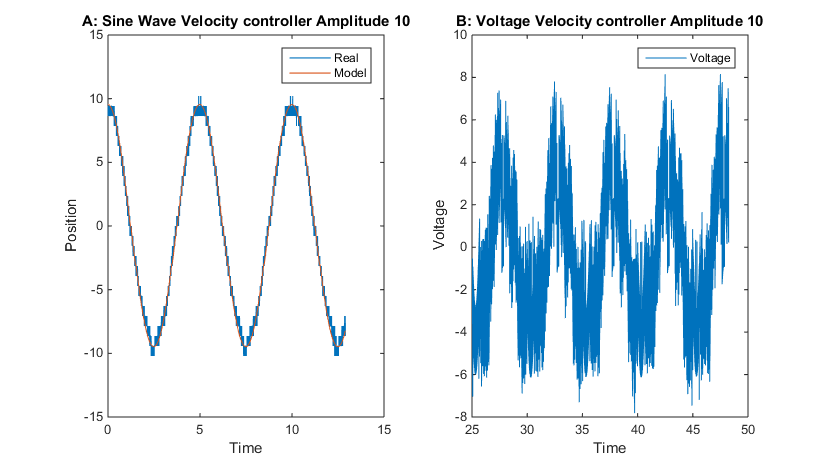
\includegraphics[scale=0.5]{41SiVo.png}
        \caption{A: Sine wave response, B: Voltage}
        \label{fig:41SiVo}
      \end{figure}

      \begin{figure}[H]
        \centering
        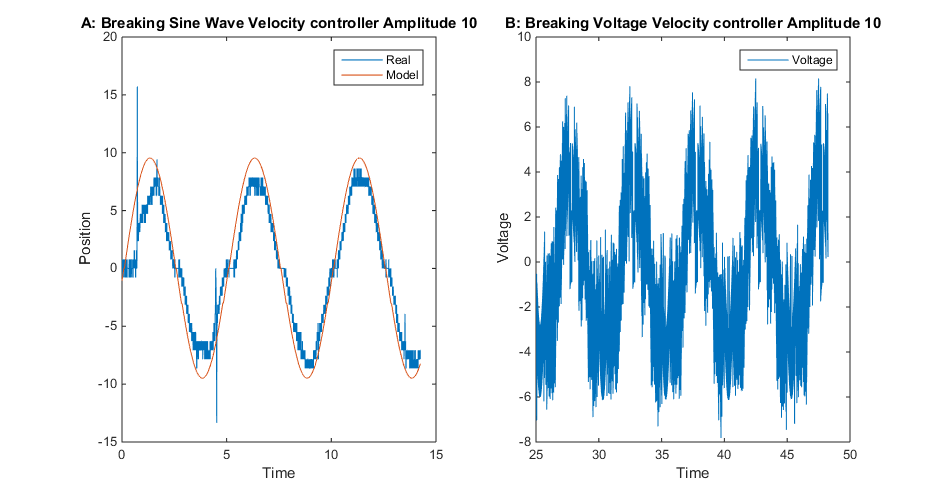
\includegraphics[scale=0.5]{41SiVoBr.png}
        \caption{A: Breaking Sine wave response, B: Voltage }
        \label{fig:41SiVoBr}
      \end{figure}
  \end{center}
 
\end{document}
